\documentclass[a4paper,12pt]{article}
\usepackage[utf8]{inputenc}
\usepackage[english]{babel}

\usepackage{siunitx}
\usepackage{graphicx}
\usepackage{amsmath}
\usepackage{hyperref}
\hypersetup{
    colorlinks=false,
    pdfborder={0 0 0},
}

\usepackage[backend=bibtex]{biblatex}
\bibliography{bibliography.bib}



\title{Some notes about subpixel accuracy}
\author{Alessandro Gentilini\thanks{alessandro.gentilini@gmail.com}}


\begin{document}
\maketitle

\begin{abstract}
Some notes about subpixel accuracy.
\end{abstract} 

\section{Some statements found in literature}
In \cite[section 8.2, p.270]{Jahne:2004:PHI:983100}:
\begin{quotation}
In order to transform images back from pixel coordinates to world coordinates,
various transformations are required. In the simplest case, this
includes only scaling,
translation (shifting), and rotation of images. More general are
affine (Section 8.3.1b)
and perspective (Section 8.3.1c) transformations. For precise
geometric measurements,
it is also required to correct for the residual geometric distortion
introduced by even
well-corrected optical systems. Modern imaging solid-state sensors are
geometrically
very precise and stable. Therefore, \textbf{the potential of a position
accuracy of better than
1/100 pixel distance is there}. To maintain this accuracy, all
geometric transformations
applied to digital images must preserve this high position accuracy.
This demand goes
far beyond the fact that no distortions are visible in the transformed images.
\end{quotation}

In \cite{halcon}:
\begin{quotation}
HALCON’s 3D calibration supports both area and line scan cameras and
permits, for example, \textbf{subpixel-accurate measurements up to \SI{1}{\micro\metre} in a field of
view of 10 mm}.
\end{quotation}

In \cite{Heikkila:2000:GCC:354167.354171}:
\begin{quotation}
Modern CCD cameras are \textbf{usually capable of a spatial accuracy greater than 1/50 of the pixel
size}. However, such accuracy is not easily attained due to various error sources that can affect
the image formation process.
\end{quotation}

In \cite{Fisher}:
\begin{quotation}
A \textbf{commonly quoted rule of thumb is 0.1 pixel}, but lower is achievable, e.g. \textbf{about 0.02 pixel is shown for stripe position detection} in [1]\footnote{Cited here as \cite{doi:10.1117/12.55947}.}.
\end{quotation}

In \cite{Davies:2012:CMV:2341317}:
\begin{quotation}
20.3.3 Differing Requirements for Size Measurement

Size measurement is important both in the food industry and in the automotive
and small-parts industry. However, the problems in the two cases are often rather
different. For example, the diameter of a biscuit can vary within quite wide limits
($\sim$5\%) without giving rise to undue problems, but when it gets outside this range,
there is a serious risk of jamming the packing machine, and the situation must be
monitored carefully. In contrast, for mechanical parts, the required precision can
vary from 1\% for objects such as O-rings to 0.01\% for piston heads. This variation
clearly makes it difficult to design a truly general-purpose inspection system.
However, the manufacturing process often permits little variation in size from one
item to the next. Hence, it may be adequate to have a system that is capable of
measuring to an accuracy of rather better than 1\%, so long as it is capable of
checking all the characteristics mentioned in Table 20.1.
For cases where high precision is vital, it is important that accuracy of measurement
is proportional to the resolution of the input image. Currently, images of
up to 512 $\times$ 512 pixels are common, so accuracy of measurement is basically of
the order of 0.2\%. Fortunately, grayscale images provide a means of obtaining
significantly greater accuracy than indicated by the above arguments, since the
exact transition from dark to light at the boundary of an object can be estimated
more closely. In addition, averaging techniques (e.g., along the side of a rectangular
block of metal) permit accuracies to be increased even further--by a factor $\sqrt{N}$
if
$N$ pixel measurements are made. These factors permit measurements to be made to
\textbf{subpixel resolution, sometimes even down to 0.1 pixels}, the limit often being set by
variations in illumination rather than by the vision algorithms themselves.
\end{quotation}

In \cite{oulu}:
\begin{quotation}
Modern CCD cameras are \textbf{usually capable of a spatial accuracy greater than 1/50 of the pixel size}. However, such accuracy is not easily attained due to various error sources that can affect the image formation process. Current calibration methods typically assume that the observations are unbiased, the only error is the zero-mean independent and identically distributed random noise in the observed image coordinates, and the camera model completely explains the mapping between the 3D coordinates and the image coordinates. In general, these conditions are not met, causing the calibration results to be less accurate than expected.
\end{quotation}

In \cite{eren2014measurement}:
\begin{quotation}
In special circumstances, measurements to subpixel accuracy can be achieved by
interpolation between pixel values, and Reference 3\footnote{Cited here as \cite{knives}.} describes the \textbf{measurement of a knife edge to about
0.1 pixel accuracy}. As a rule of thumb, however, for size measurement applications, the sensor should
have a number of pixels at least equal to twice the ratio of the largest to smallest object sizes of interest
[4]\footnote{Cited here as \cite{hopwood1980design}.}, and a lens is then selected to provide the required magnification and working distance.
\end{quotation}

In the abstract of \cite{MIKHAIL198463}:
\begin{quotation}
\textbf{Accuracies achieved have reached to within 0.03–0.05 pixel}.
\end{quotation}

\subsection{Carsten Steger's thesis}

\begin{figure}
  \centering
  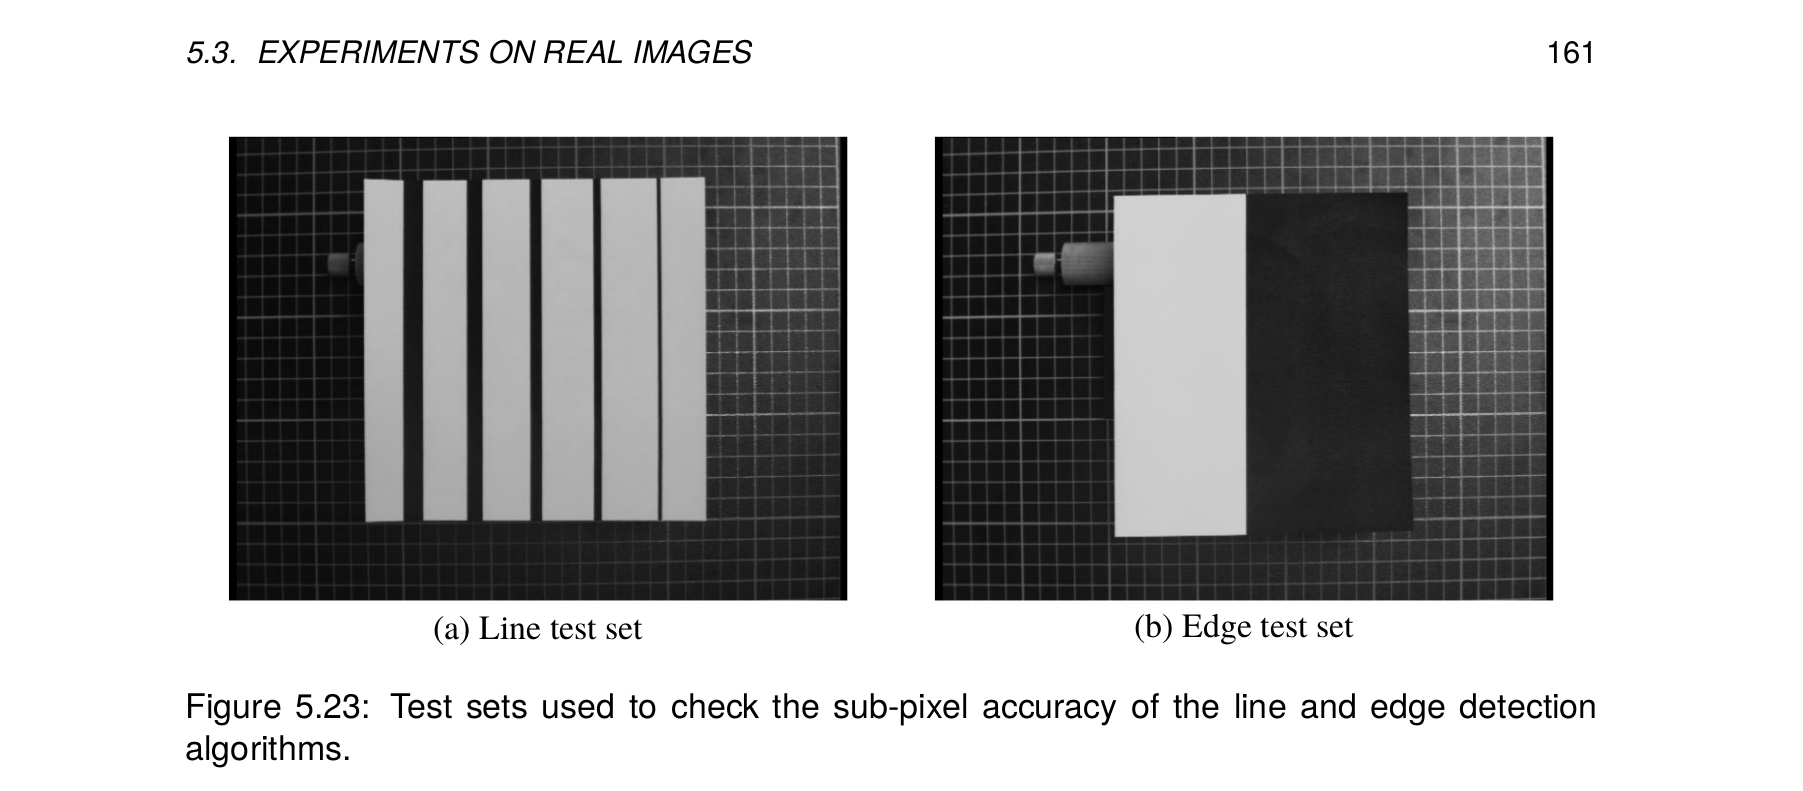
\includegraphics[width=\textwidth]{Steger_Thesis_Fig5_23}
  \caption{Figure 5.23 from Steger's thesis \cite{Steger}.}
\end{figure}

In \cite[p.1]{Steger}
\begin{quotation}
Experiments on real images
show that \textbf{sub-pixel accuracy better than one tenth of a pixel is possible in typical inspection
tasks}.
\end{quotation}

In \cite[Section 5.3.2
Sub-Pixel Accuracy of Line Position and Width, p.164]{Steger}
\begin{quotation}
Therefore, \textbf{relative shifts of one tenth of a pixel can definitively be detected
in real images.}
\end{quotation}
\begin{quotation}
As can be seen, the \textbf{absolute position errors are less than
one fortieth of a pixel.}
\end{quotation}

In \cite[Section 5.3.2
Sub-Pixel Accuracy of Line Position and Width, p.165]{Steger}
\begin{quotation}
As can be seen, the variance is less than 0.0005 almost everywhere, i.e., \textbf{the standard
deviation of the extracted line widths is less than one fortieth of a pixel.}
\end{quotation}

In \cite[5.3.3 Sub-Pixel Accuracy of Edge Position, p.166]{Steger}
\begin{quotation}
However, the standard deviation of the edge positions is still very
small, being approximately one twenty-fifth of a pixel. Therefore, with the same hypothesis
test as used above, it can be shown that \textbf{edge shifts of one tenth of a pixel can be detected with
better than 99.9\% probability.}
\end{quotation}

\begin{quotation}
\textbf{The maximum absolute error is approximately one thirtieth of a pixel.} Therefore, edges can be
extracted with very good absolute sub-pixel accuracy.
\end{quotation}

In \cite[Chapter 6 Conclusions, p.168]{Steger}
\begin{quotation}
For real images it is shown that \textbf{position shifts of one tenth of a pixel can be
detected with a probability of more than 99.9\%}, indicating that much better sub-pixel accuracy
than one tenth of a pixel can be achieved for real images. Thus, it is shown that the line and
edge extraction algorithms not only achieve sub-pixel resolution, but also sub-pixel precision
and accuracy.
\end{quotation}








\printbibliography
\end{document}
